\newpage
	\section{\Large Zielbestimmung}
	
	\subsection{Musskriterien}
	
	\subsection{Abgrenzungskriterien}

	
	\section{\Large Produkteinsatz}
	\subsection{Anwendungsbereiche}
	
	\subsection{Zielgruppen}

	\subsection{Betriebsbedingungen}

	\section{\Large Produktübersicht}
	Gibt eine Übersicht über das Produkt, z.B. über alle wichtigen Geschäftsprozesse in Form eines Übersichtsdiagramms.
	\subsection{Usecase Diagramm}
		\begin{figure}[H]
			\centering
			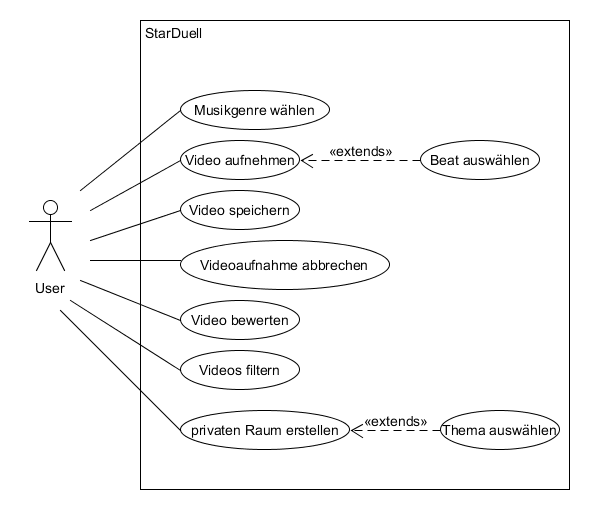
\includegraphics[width=0.7\linewidth]{images/UseCaseDiagramm}
			\caption{UseCase Diagramm}
			\label{fig:Usecase Diagramm}
		\end{figure}
		
		
	\section{\Large Produktfunktionen}
	\subsection{Usecase-Beschreibungen}
	\begin{table}[H]
		\begin{tabular}{|p{8cm}|p{8cm}|}
			\hline
			\textbf{UC-01 } \\ 
			\hline
			\textbf{ID :}\centering & UC-01  \\ \hline 
			\textbf{Title :}\centering & Video aufnehmen \\ \hline 
			\textbf{Description :}\centering & Der User startet eine Videoaufnahme \\ \hline 
			\textbf{Trigger :}\centering & User tippt auf den "play" - Button \\ \hline 
			\textbf{Primary Actor :} \centering & User \\ \hline 
			\textbf{Preconditions :}\centering & 
				\\ \hline 
			\textbf{Postconditions :}\centering &  
			 \\ \hline
			\textbf{Other Use Cases :}\centering & - \\ \hline  
			\textbf{Main Success Scenario :}\centering & 
			 \\ \hline  
			\textbf{Extensions :}\centering & \\ \hline  
			\textbf{Priority :}\centering & High \\ \hline  
		\end{tabular}
	\end{table}	
	
	\begin{table}[H]
		\begin{tabular}{|p{8cm}|p{8cm}|}
			\hline
			\textbf{UC-02 } \\ 
			\hline
			\textbf{ID :}\centering & UC-02  \\ \hline 
			\textbf{Title :}\centering & Video speichern \\ \hline 
			\textbf{Description :}\centering & User speichert das Video in der Datenbank \\ \hline 
			\textbf{Trigger :}\centering & User tippt auf den Button "Speichern" \\ \hline 
			\textbf{Primary Actor :} \centering & User \\ \hline 
			\textbf{Preconditions :}\centering & 
			\\ \hline 
			\textbf{Postconditions :}\centering & 
			 \\ \hline
			\textbf{Other Use Cases :}\centering & - \\ \hline  
			\textbf{Main Success Scenario :}\centering & 
			\\ \hline  
			\textbf{Extensions :}\centering &  \\ \hline  
			\textbf{Priority :}\centering & High \\ \hline  
		\end{tabular}
	\end{table}
	
	\begin{table}[H]
		\begin{tabular}{|p{8cm}|p{8cm}|}
			\hline
			\textbf{UC-03 } \\ 
			\hline
			\textbf{ID :}\centering & UC-03  \\ \hline 
			\textbf{Title :}\centering & Videoaufnahme abbrechen  \\ \hline 
			\textbf{Description :}\centering & Der User bricht die Videoaufnahme ab und die bisherige Aufzeichnung wird verworfen  \\ \hline 
			\textbf{Trigger :}\centering & User tippt auf Button  \\ \hline 
			\textbf{Primary Actor :} \centering & User \\ \hline 
			\textbf{Preconditions :}\centering & 
			\\ \hline 
			\textbf{Postconditions :}\centering & 
			\\ \hline
			\textbf{Other Use Cases :}\centering & - \\ \hline  
			\textbf{Main Success Scenario :}\centering & 
			 \\ \hline  
			\textbf{Extensions :}\centering &  \\ \hline  
			\textbf{Priority :}\centering & High \\ \hline  
		\end{tabular}
	\end{table}
	
	\begin{table}[H]
		\begin{tabular}{|p{8cm}|p{8cm}|}
			\hline
			\textbf{UC-04 } \\ 
			\hline
			\textbf{ID :}\centering & UC-04  \\ \hline 
			\textbf{Title :}\centering & Video bewerten \\ \hline 
			\textbf{Description :}\centering & Ein User kann ein Video bewerten \\ \hline 
			\textbf{Trigger :}\centering & User tippt auf "Stern" - Button  \\ \hline 
			\textbf{Primary Actor :} \centering & User \\ \hline 
			\textbf{Preconditions :}\centering & 
			\\ \hline 
			\textbf{Postconditions :}\centering & 
			\\ \hline
			\textbf{Other Use Cases :}\centering & - \\ \hline  
			\textbf{Main Success Scenario :}\centering & 
			\\ \hline  
			\textbf{Extensions :}\centering & 
			\\ \hline  
			\textbf{Priority :}\centering & High \\ \hline  
		\end{tabular}
	\end{table}
	
	\begin{table}[H]
		\begin{tabular}{|p{8cm}|p{8cm}|}
			\hline
			\textbf{UC-05 } \\ 
			\hline
			\textbf{ID :}\centering & UC-05  \\ \hline 
			\textbf{Title :}\centering & Video filtern \\ \hline 
			\textbf{Description :}\centering & Dem User werden die Videos nach einem bestimmten Filter aufgelistet \\ \hline 
			\textbf{Trigger :}\centering & User bestimmt Filter und tippt auf Button \\ \hline 
			\textbf{Primary Actor :} \centering & User \\ \hline 
			\textbf{Preconditions :}\centering & 
			\\ \hline 
			\textbf{Postconditions :}\centering &
			\\ \hline
			\textbf{Other Use Cases :}\centering & - \\ \hline  
			\textbf{Main Success Scenario :}\centering &
			\\ \hline  
			\textbf{Extensions :}\centering &  \\ \hline  
			\textbf{Priority :}\centering & High \\ \hline  
		\end{tabular}
	\end{table}	
	
	\begin{table}[H]
		\begin{tabular}{|p{8cm}|p{8cm}|}
			\hline
			\textbf{UC-06 } \\ 
			\hline
			\textbf{ID :}\centering & UC-06  \\ \hline 
			\textbf{Title :}\centering & Musikgenre wählen \\ \hline 
			\textbf{Description :}\centering & Der User bestimmt das Musikgenre seines Videos \\ \hline 
			\textbf{Trigger :}\centering & User wählt aus einer Liste das Genre und bestätigt es mit einem Button \\ \hline 
			\textbf{Primary Actor :} \centering & User \\ \hline 
			\textbf{Preconditions :}\centering &\\ \hline 
			\textbf{Postconditions :}\centering	& 
			\\ \hline		
			\textbf{Other Use Cases :}\centering & - \\ \hline  
			\textbf{Main Success Scenario :}\centering &
			\\ \hline  
			\textbf{Extensions :}\centering & - \\ \hline  
			\textbf{Priority :}\centering & High \\ \hline  
		\end{tabular}
	\end{table}

	\begin{table}[H]
		\begin{tabular}{|p{8cm}|p{8cm}|}
			\hline
			\textbf{UC-07 } \\ 
			\hline
			\textbf{ID :}\centering & UC-07  \\ \hline 
			\textbf{Title :}\centering & privaten Raum erstellen \\ \hline 
			\textbf{Description :}\centering &  \\ \hline 
			\textbf{Trigger :}\centering & User klickt auf den Button "'Speichern Unter"' \\ \hline 
			\textbf{Primary Actor :} \centering & User \\ \hline 
			\textbf{Preconditions :}\centering & \\ \hline 
			\textbf{Postconditions :}\centering	& 
			\\ \hline		
			\textbf{Other Use Cases :}\centering & - \\ \hline  
			\textbf{Main Success Scenario :}\centering &
			\\ \hline  
			\textbf{Extensions :}\centering & \\ \hline  
			\textbf{Priority :}\centering & High \\ \hline  
		\end{tabular}
	\end{table}			
	
	\subsection{Aktivitätsdiagramm}

	\subsection{Sequenzdiagramm}
	
	
\newpage
	\section{\Large Produktdaten}
	
	\subsection{Analyseklassendiagramm}	
	
	\subsection{Paketdiagramm}
	
	\subsection{Domänenklassendiagramm}
	
	\section{\Large Produktleistungen}
	
	\section{\Large Qualitätsanforderungen}
	
	
	\section{\Large Benutzeroberfläche}
	
	\subsection{Zustandsdiagramme}
	
	\section{\Large Nichtfunktionale Anforderungen}
	

	
	\section{\Large Technische Produktumgebung}
   	In diesem Kapitel wird die technische Umgebung des Produkts beschrieben.\\
   	Bei Client / Server-Anwendungen ist die Umgebung jeweils für Clients und Server getrennt anzugeben.
	\subsection{Software}
	
	\subsection{Hardware}
	
	\subsection{Orgware}
	
	\subsection{Produkt-Schnittstellen}

	
	\section{\Large Spezielle Anforderungen an die Entwicklungs-Umgebung}
	
	\subsection{Software}
	\subsection{Hardware}
	\subsection{Orgware}
	\subsection{Entwicklungsschnittstellen}
	
	
	\section{\Large Gliederung in Teilprodukte}
	
	
	\section{\Large Ergänzungen}
	.
	
\newpage
	\section{\Large Glossar}
	In diesem Kapitel wird die spezifische Sprache des Auftraggebers wie \textbf{ Kürzel } und \textbf{ Fachbegriffe } beschrieben, z.B. :
	
		
		